% 2008 年湖北卷文科第 5 题：不等式组 |x|<=|y|、|x|<1 所表示区域的四个候选图。
% 来源 PDF：gaokaomath-src/普通高考/2008/2008湖北文.pdf
% SHA-256：e097163e244cb8f03775ac7ff2e344ef85471e91ecc717d23698a0fb01e76963
% 原页：2008湖北文.pdf 第 1 页（A3 三栏）第 1 栏，书页码 451。
% 绘制依据：四个候选按原页排成 2×2——
%   (A) |x|<=|y| 且 |y|<=1（上下两个三角，横向虚线 y=±1）；
%   (B) y>=|x| 且 |x|<1（上方楔形，竖向虚线 x=±1）；
%   (C) |x|<=|y| 且 |x|<1（上下两个楔形，竖向虚线 x=±1）——即题设区域；
%   (D) |y|<=|x| 且 |x|<1（左右两个楔形，竖向虚线 x=±1）。
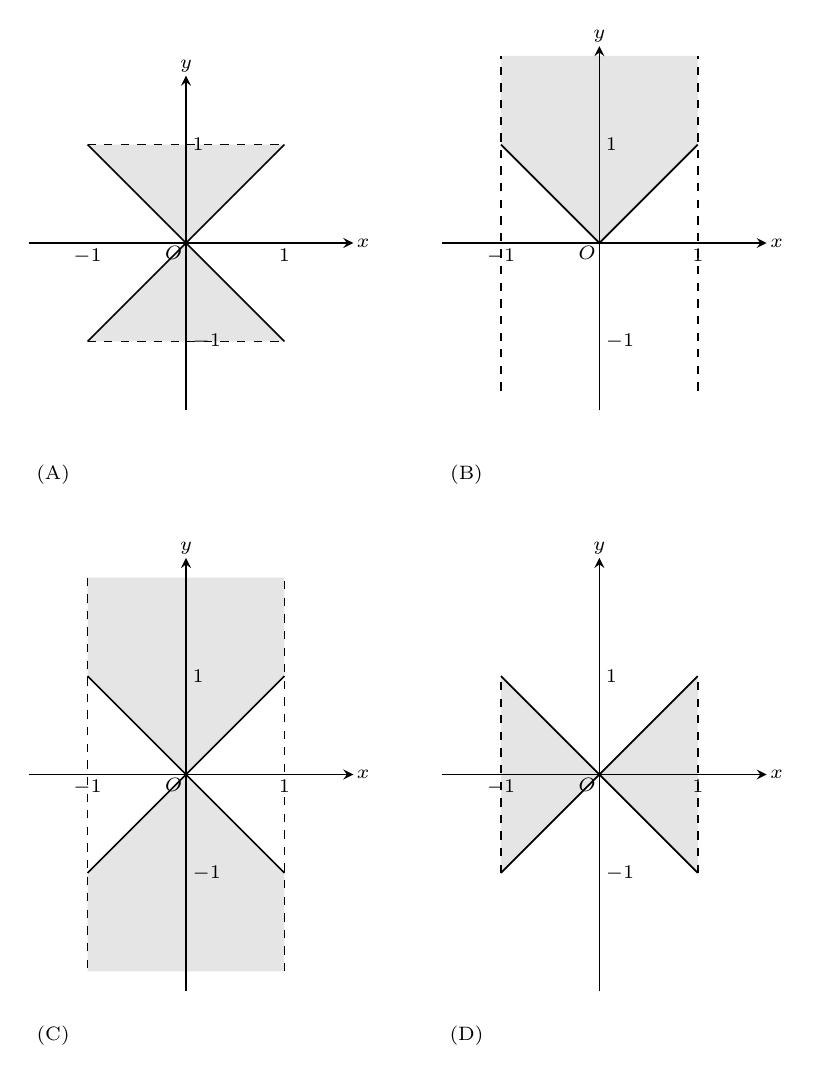
\begin{tikzpicture}[x=1.25cm, y=1.25cm, semithick, font=\scriptsize,
  every node/.style={inner sep=1.0pt}]

  % ---------- (A) |x|<=|y|<=1 ----------
  \begin{scope}[shift={(0,0)}]
    \fill[gray!20] (-1,1) -- (0,0) -- (1,1) -- cycle;
    \fill[gray!20] (-1,-1) -- (0,0) -- (1,-1) -- cycle;
    \draw[->,>=stealth] (-1.6,0) -- (1.7,0) node[right] {$x$};
    \draw[->,>=stealth] (0,-1.7) -- (0,1.7) node[above] {$y$};
    \node[below left] at (0,0) {$O$};
    \draw[dashed] (-1,1) -- (1,1);
    \draw[dashed] (-1,-1) -- (1,-1);
    \draw (-1,1) -- (0,0) -- (1,1);
    \draw (-1,-1) -- (0,0) -- (1,-1);
    \node[below] at (-1,-0.02) {$-1$};
    \node[below] at (1,-0.02) {$1$};
    \node[right] at (0.03,1) {$1$};
    \node[right] at (0.03,-1) {$-1$};
    \node at (-1.35,-2.35) {(A)};
  \end{scope}

  % ---------- (B) y>=|x|, |x|<1 ----------
  \begin{scope}[shift={(4.2,0)}]
    \fill[gray!20] (-1,1) -- (-1,1.9) -- (1,1.9) -- (1,1) -- (0,0) -- cycle;
    \draw[->,>=stealth] (-1.6,0) -- (1.7,0) node[right] {$x$};
    \draw[->,>=stealth] (0,-1.7) -- (0,2.0) node[above] {$y$};
    \node[below left] at (0,0) {$O$};
    \draw[dashed] (-1,-1.5) -- (-1,1.9);
    \draw[dashed] (1,-1.5) -- (1,1.9);
    \draw (-1,1) -- (0,0) -- (1,1);
    \node[below] at (-1,-0.02) {$-1$};
    \node[below] at (1,-0.02) {$1$};
    \node[right] at (0.03,1) {$1$};
    \node[right] at (0.03,-1) {$-1$};
    \node at (-1.35,-2.35) {(B)};
  \end{scope}

  % ---------- (C) |x|<=|y|, |x|<1 ----------
  \begin{scope}[shift={(0,-5.4)}]
    \fill[gray!20] (-1,1) -- (-1,2.0) -- (1,2.0) -- (1,1) -- (0,0) -- cycle;
    \fill[gray!20] (-1,-1) -- (-1,-2.0) -- (1,-2.0) -- (1,-1) -- (0,0) -- cycle;
    \draw[->,>=stealth] (-1.6,0) -- (1.7,0) node[right] {$x$};
    \draw[->,>=stealth] (0,-2.2) -- (0,2.2) node[above] {$y$};
    \node[below left] at (0,0) {$O$};
    \draw[dashed] (-1,2.0) -- (-1,-2.0);
    \draw[dashed] (1,-2.0) -- (1,2.0);
    \draw (-1,1) -- (0,0) -- (1,1);
    \draw (-1,-1) -- (0,0) -- (1,-1);
    \node[below] at (-1,-0.02) {$-1$};
    \node[below] at (1,-0.02) {$1$};
    \node[right] at (0.03,1) {$1$};
    \node[right] at (0.03,-1) {$-1$};
    \node at (-1.35,-2.65) {(C)};
  \end{scope}

  % ---------- (D) |y|<=|x|, |x|<1 ----------
  \begin{scope}[shift={(4.2,-5.4)}]
    \fill[gray!20] (-1,1) -- (-1,-1) -- (0,0) -- cycle;
    \fill[gray!20] (1,1) -- (1,-1) -- (0,0) -- cycle;
    \draw[->,>=stealth] (-1.6,0) -- (1.7,0) node[right] {$x$};
    \draw[->,>=stealth] (0,-2.2) -- (0,2.2) node[above] {$y$};
    \node[below left] at (0,0) {$O$};
    \draw[dashed] (-1,-1) -- (-1,1);
    \draw[dashed] (1,-1) -- (1,1);
    \draw (-1,1) -- (0,0) -- (-1,-1);
    \draw (1,1) -- (0,0) -- (1,-1);
    \node[below] at (-1,-0.02) {$-1$};
    \node[below] at (1,-0.02) {$1$};
    \node[right] at (0.03,1) {$1$};
    \node[right] at (0.03,-1) {$-1$};
    \node at (-1.35,-2.65) {(D)};
  \end{scope}
\end{tikzpicture}
